\documentclass[tikz,border=8pt]{standalone}
% Shared look for every TikZ diagram. Load with \input{../../tools/tikz-style.tex}
\usepackage[T1]{fontenc}
\usepackage{lmodern}
\renewcommand{\sfdefault}{lmr}  % diagrams use the same serif as the text
\usetikzlibrary{arrows.meta, positioning, shapes.geometric, calc, fit, backgrounds}
\definecolor{cblue}{HTML}{4C78A8}
\definecolor{corange}{HTML}{F58518}
\definecolor{cgreen}{HTML}{54A24B}
\definecolor{cred}{HTML}{E45756}
\definecolor{cpurple}{HTML}{B279A2}
\definecolor{cgrey}{HTML}{6B6B6B}
\tikzset{
  every picture/.style={font=\sffamily, line width=1.2pt},
  box/.style={draw=#1, fill=#1!12, rounded corners=4pt, align=center, inner sep=7pt, minimum height=1.1cm},
  box/.default=cgrey,
  arrow/.style={-{Stealth[length=3mm]}, draw=cgrey, line width=1.4pt},
  title/.style={font=\sffamily\bfseries\Large},
  note/.style={font=\sffamily\small, text=cgrey, align=center},
}
\AtBeginDocument{\hyphenpenalty=10000 \exhyphenpenalty=10000}

\begin{document}
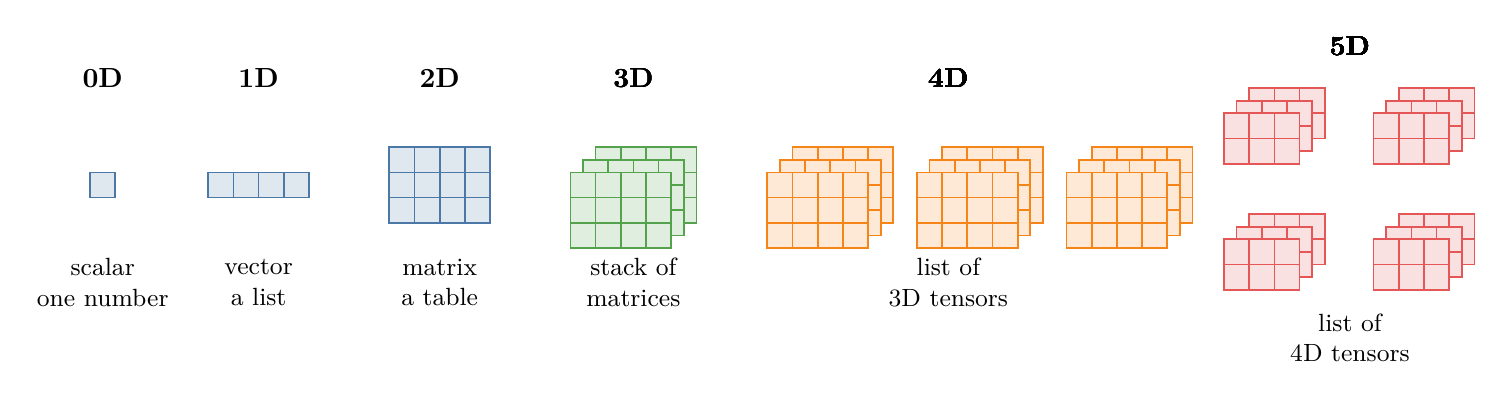
\begin{tikzpicture}[s/.style={draw=#1, fill=#1!18, line width=0.6pt}]
  % \grid{x}{y}{rows}{cols}{colour}: a grid of cells, top-left at (x,y), cell size 0.32
  \newcommand{\grid}[5]{\foreach \r in {1,...,#3} \foreach \c in {1,...,#4}
      \filldraw[s=#5] ({#1+(\c-1)*0.32},{#2-(\r-1)*0.32}) rectangle ++(0.32,-0.32);}
  % \stack{x}{y}{depth}{rows}{cols}{colour}: matrices stacked with a diagonal offset
  \newcommand{\stack}[6]{\foreach \d in {#3,...,1} \grid{#1+(\d-1)*0.16}{#2+(\d-1)*0.16}{#4}{#5}{#6}}
  \grid{0}{0}{1}{1}{cblue}
  \node[title, font=\sffamily\bfseries] at (0.16,1.2) {0D};
  \node[note, text=black, align=center] at (0.16,-1.4) {scalar\\{\small one number}};
  \grid{1.5}{0}{1}{4}{cblue}
  \node[font=\bfseries] at (2.14,1.2) {1D};
  \node[note, text=black, align=center] at (2.14,-1.4) {vector\\{\small a list}};
  \grid{3.8}{0.32}{3}{4}{cblue}
  \node[font=\bfseries] at (4.44,1.2) {2D};
  \node[note, text=black, align=center] at (4.44,-1.4) {matrix\\{\small a table}};
  \stack{6.1}{0.0}{3}{3}{4}{cgreen}
  \node[font=\bfseries] at (6.9,1.2) {3D};
  \node[note, text=black, align=center] at (6.9,-1.4) {stack of\\matrices};
  \foreach \k in {0,1,2} \stack{8.6+\k*1.9}{0.0}{3}{3}{4}{corange}
  \node[font=\bfseries] at (10.9,1.2) {4D};
  \node[note, text=black, align=center] at (10.9,-1.4) {list of\\3D tensors};
  \foreach \row in {0,1} \foreach \k in {0,1} \stack{14.4+\k*1.9}{0.75-\row*1.6}{3}{2}{3}{cred}
  \node[font=\bfseries] at (16.0,1.6) {5D};
  \node[note, text=black, align=center] at (16.0,-2.1) {list of\\4D tensors};
\end{tikzpicture}
\end{document}
